\documentclass[a4paper,12pt]{article}
\usepackage{graphicx}
\usepackage{float}
\usepackage{listings}
\usepackage{amsmath}
\usepackage{hyperref}
\graphicspath{{figures/}}
\setlength{\parindent}{0pt}

\begin{document}

    \title{Computational Biomaterials and Biomechanics\\[1ex]
    \Large Finite Element Analysis of Proximal Femur under Load}
    \author{Robin Steiner (11778873)}
    \date{\today}
    \maketitle

    \thispagestyle{empty}
    \newpage

    \tableofcontents

    \newpage


    \section{Introduction}\label{sec:introduction}
    This report focuses on the biomechanical analysis of the proximal femur, a critical aspect in understanding bone health and the impact of various load conditions, especially in the field of orthopedic research and clinical practice.
    Utilizing advances in 3D medical imaging, this analysis employs Finite Element (FE) modeling to simulate the stress distribution within the femur under typical loading conditions, such as those encountered during standing.

    \vspace{10pt}
    The motivation for this analysis stems from the need to comprehend the biomechanical behavior of the femur under load, which is essential for diagnosing and treating bone-related health issues.
    Computational models such as these play a crucial role in understanding the properties of bones, as they provide valuable insights without necessitating physical load testing, which is unfeasible for living patients.

    \vspace{10pt}
    The primary objectives of this study include generating an accurate FE model of the proximal femur based on a 3D medical image, evaluating the stress distribution under load, and assessing key parameters such as the spring stiffness of the entire femur and the displacements of the femoral head in x- and y-directions.

    \vspace{10pt}
    A 3D representation of the CT scan is shown in Figure~\ref{fig:data}

    \begin{figure}[htbp]
        \centering
        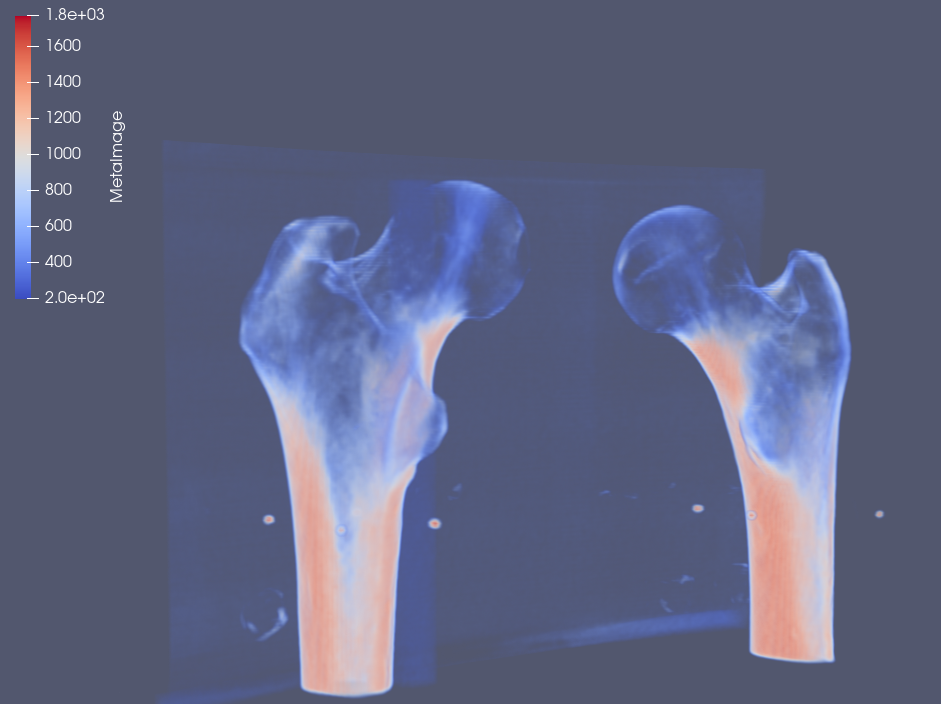
\includegraphics[width=0.7\textwidth]{data}
        \caption{CT scan of the proximal femur (3D)}
        \label{fig:data}
    \end{figure}


    \section{Methods}
    This section outlines the procedures used to create and analyze the finite element model of the proximal femur, detailing the steps from data processing to computational modeling and analysis.
    The data is pre-processed using \texttt{medtool 4.7}.
    All 3D visualizations are done with \texttt{ParaView 5.12.0}.

    \subsection{Data Preparation}\label{subsec:data-preparation}
    The first step was, to get an overview over the CT scan which serves as a basis for the analysis.
    This was done, using \texttt{ParaView}, where the result is shown Figure~\ref{fig:data}.
    The grey value threshold had to be adjusted slightly, to get a good view of the bones.
    This can also be seen in the scale on the left.

    \vspace{10pt}
    Additionally, \texttt{medtool} was used to obtain a projection along all three directions using the \texttt{mic:-proj} function.
    The contrast was adjusted slightly and the result can be seen in Figure~\ref{fig:projected}

    \begin{figure}[htbp]
        \centering
        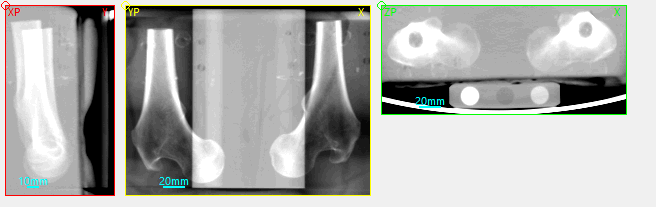
\includegraphics[width=\textwidth]{projected}
        \caption{Projected CT scan of the proximal femur (projected in X direction)}
        \label{fig:projected}
    \end{figure}

    In the next step, this projection was used to find coordinates along which the left bone can be cut out.
    This was done using the region of interest (ROI) feature in \texttt{medtool}, and the actual cut was performed using \texttt{mic:-cut}.
    As can be seen in Figure~\ref{fig:bone_cut}, a few millimeters of the shaft were cut of, to ensure a clean edge for the FE model later on.

    \begin{figure}[htbp]
        \centering
        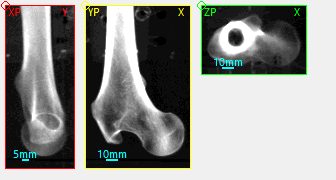
\includegraphics[width=0.7\textwidth]{bone_cut}
        \caption{Cut of the left proximal femur}
        \label{fig:bone_cut}
    \end{figure}

    A second cut was done in a similar manner, to extract the calibration phantom.
    The result can be seen in Figure~\ref{fig:phantom_cut}.

    \begin{figure}[htbp]
        \centering
        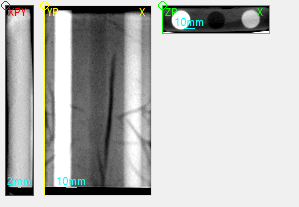
\includegraphics[width=0.7\textwidth]{phantom_cut}
        \caption{Cut of the calibration phantom}
        \label{fig:phantom_cut}
    \end{figure}

    For both cuts, the \texttt{mic:-form} was set to \texttt{int32} to save some memory compared to \texttt{float32}.

    \subsection{Calibration}\label{subsec:calibration}
    All previously obtained results are not calibrated yet.
    So the next step is to use calibration phantom cut to calibrate the bone cut.
    This step can also be done using \texttt{medtool} with the \texttt{mic:-labvox} function.
    However, since it has to be done three times for each phantom chamber, the Multi Run feature (\texttt{mic:-mfil}) can be used.
    It allows to run the labeling process three times and combining it in one output.

    \vspace{10pt}
    The \texttt{mic:-labvox} function takes a list of parameters, the first two specify which grey value the ROI selection as well as the background should be assigned to.
    The rest of the parameters specify the ROI.
    The full list of input parameters for the \texttt{mic:-mfil} function can be seen in Table~\ref{table:multi_run}.

    \begin{table}[h]
        \centering
        \begin{tabular}{|l|l|}
            \hline
            \textbf{Option} & \textbf{Value(s)}             \\
            \hline
            labvox          & 0;1-47; 10; 11; 14; 11; 170   \\
            \hline
            labvox          & None;2-82; 8; 11; 14; 12; 170 \\
            \hline
            labvox          & None;3-12, 8; 11; 13; 12; 170 \\
            \hline
            out             & exa\_labels.mhd               \\
            \hline
            mid             & exa\_labels.png               \\
            \hline
        \end{tabular}
        \caption{Input Parameters for the Multi Run, which does the labeling for calibration}
        \label{table:multi_run}
    \end{table}

    The result can be seen in Figure~\ref{fig:exa_lables} and~\ref{fig:exa_lables_3d}.

    \begin{figure}[htbp]
        \centering
        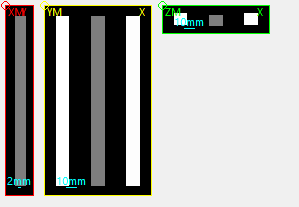
\includegraphics[width=0.7\textwidth]{exa_lables}
        \caption{Phantom chamber cut-outs for calibration}
        \label{fig:exa_lables}
    \end{figure}

    \begin{figure}[htbp]
        \centering
        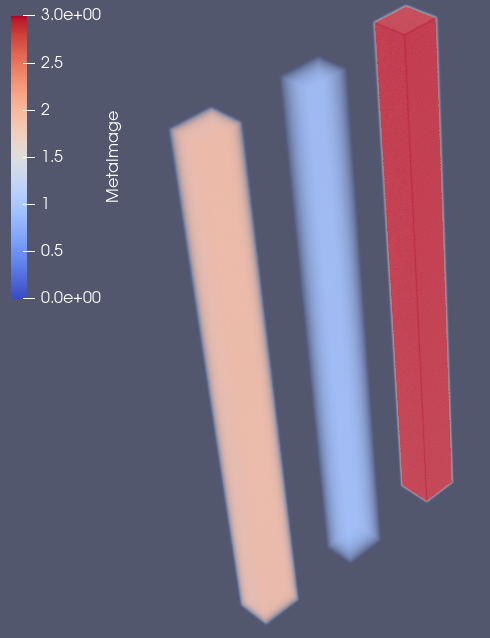
\includegraphics[width=0.5\textwidth]{exa_lables_3d}
        \caption{3D representation of the phantom chamber cut-outs for calibration}
        \label{fig:exa_lables_3d}
    \end{figure}

    Using those labels the actual calibration of the bone cut-out can be performed.
    Within \texttt{medtool} a calibration script was created, with the original phantom cut (\texttt{-inp}), the labelled phantom (\texttt{-inl}) and the bone cut (\texttt{-inc}) as input files.
    Additionally, the tissue densities of the phantom chambers are defined as 0, 100 and 200 mgHA/ccm (\texttt{-tiss}).
    Lastly the minimal and maximal density are set to 0 and 1060 (\texttt{-limit}).

    \vspace{10pt}
    The resulting calibration curve, as well as the calibrated bone can be seen in Figure~\ref{fig:calibration_curve} and~\ref{fig:bone_calibrated}.

    \begin{figure}[htbp]
        \centering
        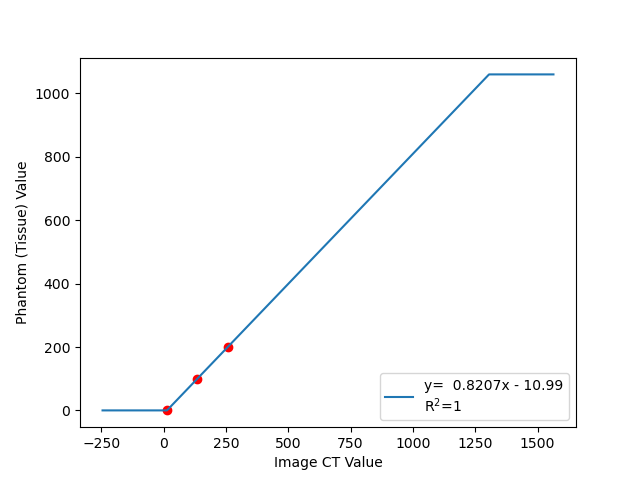
\includegraphics[width=0.7\textwidth]{calibration_curve}
        \caption{Calibration regression curve}
        \label{fig:calibration_curve}
    \end{figure}

    \begin{figure}[htbp]
        \centering
        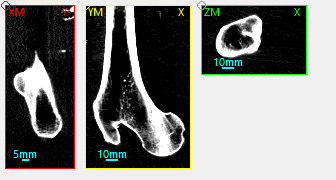
\includegraphics[width=0.7\textwidth]{bone_calibrated}
        \caption{Calibrated image of the bone}
        \label{fig:bone_calibrated}
    \end{figure}

    \subsection{Resolution and Scaling}\label{subsec:resolution-and-scaling}
    For now there is too much information in our bone sample to be transformed into an FE model.
    The function \texttt{mic:-resf} can be used to change the resolution by a given factor, in this case the factor 3 was used.
    Using the \texttt{mic:-scale} function the gray value range was additionally reduced to 0--250.
    Due to this lower range, the \texttt{mic:-form} could be changed to \texttt{uint8} to save on memory.
    The resulting midplanes of this lower resolution bone can be seen in Figures~\ref{fig:bone_low_res-XM}-\ref{fig:bone_low_res-ZM}

    \begin{figure}[htbp]
        \centering
        \begin{minipage}[b]{0.3\textwidth}
            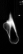
\includegraphics[width=0.7\textwidth]{bone_low_res-XM}
            \caption{Reduced resolution of the bone for FE (X-midplane)}
            \label{fig:bone_low_res-XM}
        \end{minipage}
        \hfill
        \begin{minipage}[b]{0.3\textwidth}
            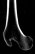
\includegraphics[width=0.7\textwidth]{bone_low_res-YM}
            \caption{Reduced resolution of the bone for FE (Y-midplane)}
            \label{fig:bone_low_res-YM}
        \end{minipage}
        \hfill
        \begin{minipage}[b]{0.3\textwidth}
            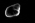
\includegraphics[width=0.7\textwidth]{bone_low_res-ZM}
            \caption{Reduced resolution of the bone for FE (Z-midplane)}
            \label{fig:bone_low_res-ZM}
        \end{minipage}
    \end{figure}

    \subsection{Masking}\label{subsec:masking}

    The next step is to mask the bone, in order to remove background artifacts.
    The function \texttt{mic:-clean} can be used for this.
    A second step the \texttt{mic:-fill} function with a threshold value 10 was employed, to create a segmented image of the bone.
    Finally, \texttt{mic:-scale} was used in an additional step to reduce the values of the mask to 0 for the background and 1 for the bone.
    The produced mask can be seen in Figure~\ref{fig:scale_mask-XM}-\ref{fig:scale_mask-ZM}
    \begin{figure}[htbp]
        \centering
        \begin{minipage}[b]{0.3\textwidth}
            
\includegraphics[width=0.7\textwidth]{scale_mask-XM}
            \caption{Mask for the bone (X-midplane)}
            \label{fig:scale_mask-XM}
        \end{minipage}
        \hfill
        \begin{minipage}[b]{0.3\textwidth}
            
\includegraphics[width=0.7\textwidth]{scale_mask-YM}
            \caption{Mask for the bone (Y-midplane)}
            \label{fig:scale_mask-YM}
        \end{minipage}
        \hfill
        \begin{minipage}[b]{0.3\textwidth}
            
\includegraphics[width=0.7\textwidth]{scale_mask-ZM}
            \caption{Mask for the bone (Z-midplane)}
            \label{fig:scale_mask-ZM}
        \end{minipage}
    \end{figure}

    To apply this mask to the bone \texttt{mic:-mask} was used.
    The result is shown in Figures~\ref{fig:bone_masked-XM}-\ref{fig:bone_masked-ZM}

    \begin{figure}[htbp]
        \centering
        \begin{minipage}[b]{0.3\textwidth}
            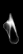
\includegraphics[width=0.7\textwidth]{bone_masked-XM}
            \caption{Masked bone (X-midplane)}
            \label{fig:bone_masked-XM}
        \end{minipage}
        \hfill
        \begin{minipage}[b]{0.3\textwidth}
            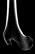
\includegraphics[width=0.7\textwidth]{bone_masked-YM}
            \caption{Masked bone (Y-midplane)}
            \label{fig:bone_masked-YM}
        \end{minipage}
        \hfill
        \begin{minipage}[b]{0.3\textwidth}
            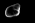
\includegraphics[width=0.7\textwidth]{bone_masked-ZM}
            \caption{Masked bone (Z-midplane)}
            \label{fig:bone_masked-ZM}
        \end{minipage}
    \end{figure}

    \subsection{Embedding}\label{subsec:embedding}
    As a final step before the FE model can be created, an embedding around the femoral head is added, upon which load can be applied.
    For this the \texttt{mic:-embed} function was used with the following parameter list: 3;6;0;255, where 3 represents the z-direction, 6 and 0 are the values for \texttt{thickVoxIn} and \texttt{thickVoxOut}, which give the thickness of the embedding layer inside and outside of a bounding box.
    Finally, 255 is the new grey value applied to the embedding.
    The result is shown in Figure~\ref{fig:bone_embedded-XM}-\ref{fig:bone_embedded-ZM} as well as a 3D depection in Figure~\ref{fig:bone_embedded}.

    \begin{figure}[htbp]
        \centering
        \begin{minipage}[b]{0.3\textwidth}
            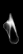
\includegraphics[width=0.7\textwidth]{bone_embedded-XM}
            \caption{Final masked bone with embedding at head (X-midplane)}
            \label{fig:bone_embedded-XM}
        \end{minipage}
        \hfill
        \begin{minipage}[b]{0.3\textwidth}
            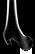
\includegraphics[width=0.7\textwidth]{bone_embedded-YM}
            \caption{Final masked bone with embedding at head (Y-midplane)}
            \label{fig:bone_embedded-YM}
        \end{minipage}
        \hfill
        \begin{minipage}[b]{0.3\textwidth}
            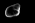
\includegraphics[width=0.7\textwidth]{bone_embedded-ZM}
            \caption{Final masked bone with embedding at head (Z-midplane)}
            \label{fig:bone_embedded-ZM}
        \end{minipage}
    \end{figure}

    \begin{figure}[htbp]
        \centering
        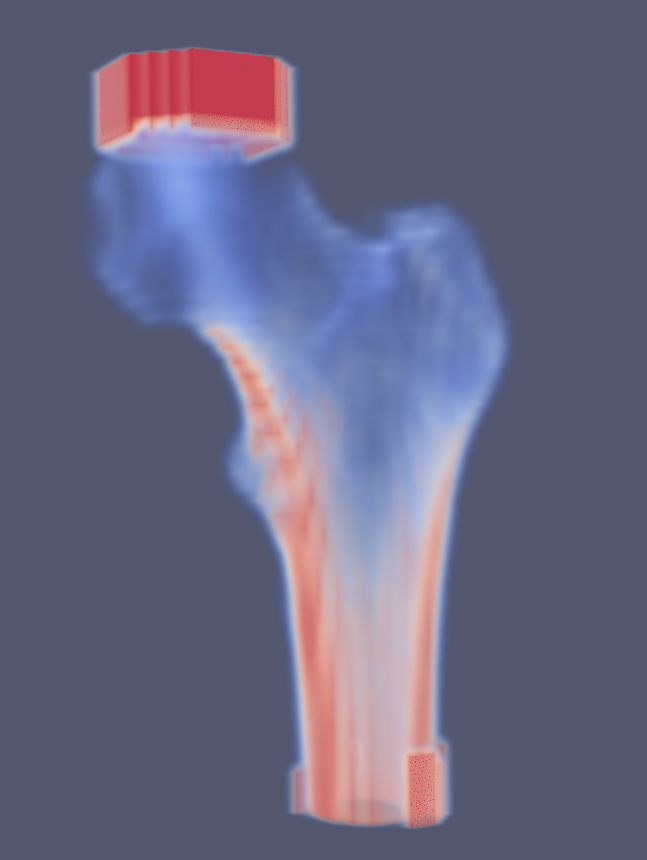
\includegraphics[width=0.5\textwidth]{bone_embedded}
        \caption{Final masked bone with embedding at head (3D)}
        \label{fig:bone_embedded}
    \end{figure}

    \subsection{Finite Element Analysis}\label{subsec:model-generation}
    Now the bone can be used as a basis to generate a FE model.
    Again \texttt{medtool} provides a script for this, which generates a \texttt{.inp} file, that can be interpreted by different FE solvers.
    As an input this script takes the bone that was prepared in the previous steps, the material properties associated with the elements, as well as boundary conditions.

    \vspace{10pt}
    For the embedding an elastic standard material with $E = 2200 MPa$ and $\nu = 0.3$ is used.
    For the bone itself an elastic power law $E_0 = 5000 MPa$ and $\nu = 0.3$ $k = 2.5$ is used.

    \vspace{10pt}
    For the boundary conditions, the distal end of the femoral shaft was fixed, meaning that no displacement is allowed there.
    At the embedding, only the z-direction is fixed and set to a constant value of $z_{disp} = -0.3 mm$.
    In \texttt{medtool} this can be achieved by setting the \texttt{-disp} option to \texttt{ALL\_NODE \_B;1-3;0.0;ALL\_NODE\_T;3;-0.3}.
    Note, that for this to work, the \texttt{-nsetfa} option has to be turned on additionally, which creates the node sets for \texttt{ALL\_NODE\_B} (all nodes at the bottom) and \texttt{ALL\_NODE\_T} (all nodes at the top).

    Finally, this model generated \texttt{.inp} is run with \texttt{Calcullix}.


    \section{Results}\label{sec:results}
    I this section the key findings from the finite element analysis, including stress distribution, femoral head displacements, and femur spring stiffness are presented.

    \vspace{10pt}
    Figure~\ref{fig:model} and~\ref{fig:model_cut} show the generated FE model with its nodes.
    Each color represents a different material with a different Young's modulus according to the power law.

    \begin{figure}[htbp]
        \centering
        \begin{minipage}[b]{0.49\textwidth}
            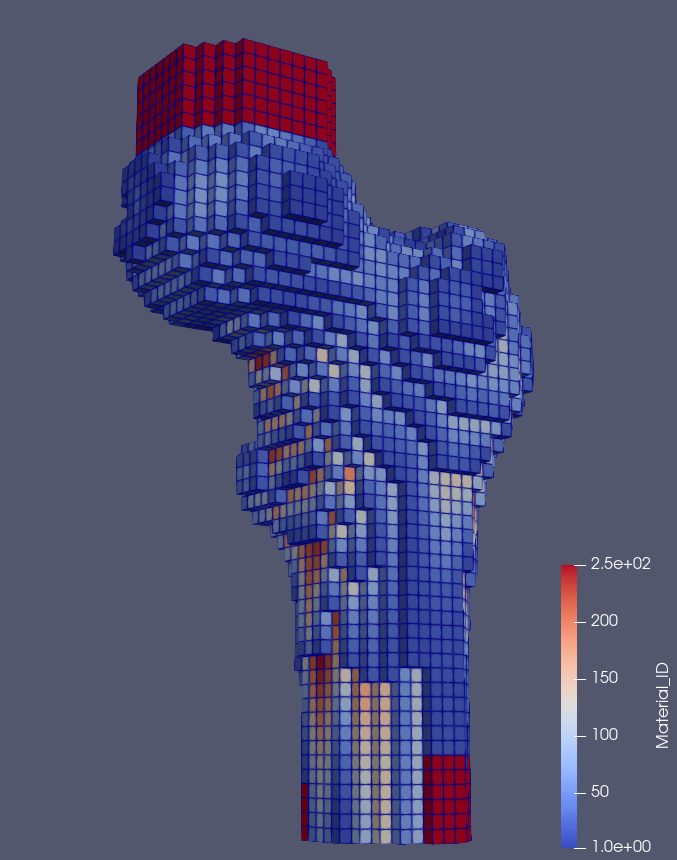
\includegraphics[width=\textwidth]{model}
            \caption{3D representation of the FE model with different colors representing different material properties}
            \label{fig:model}
        \end{minipage}
        \hfill
        \begin{minipage}[b]{0.49\textwidth}
            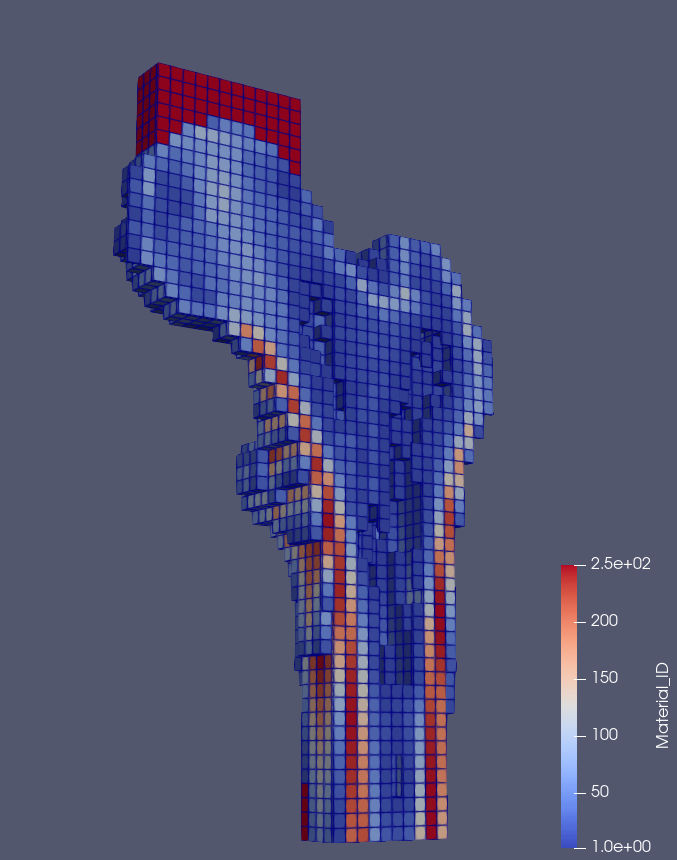
\includegraphics[width=\textwidth]{model_cut}
            \caption{Clipped version of the FE model with different colors representing different material properties}
            \label{fig:model_cut}
        \end{minipage}
    \end{figure}

    \vspace{10pt}
    Figures~\ref{fig:displacement-X}-\ref{fig:displacement-Z} illustrate the displacement magnitudes in different directions.
    All use the same scale, to highlight the relative differences between them as well.
    Figure~\ref{fig:displacement} shows the summed up magnitude of the displacement in each node.
    The bone was cut in half for all of those illustration.

    \begin{figure}[htbp]
        \centering
        \begin{minipage}[b]{0.3\textwidth}
            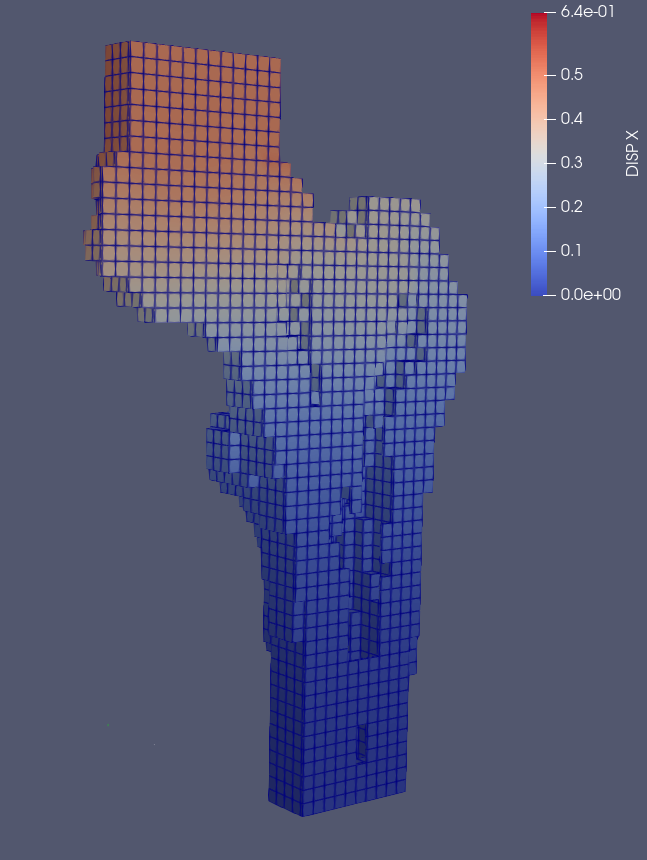
\includegraphics[width=\textwidth]{displacement-X}
            \caption{Displacement magnitude in X direction}
            \label{fig:displacement-X}
        \end{minipage}
        \hfill
        \begin{minipage}[b]{0.3\textwidth}
            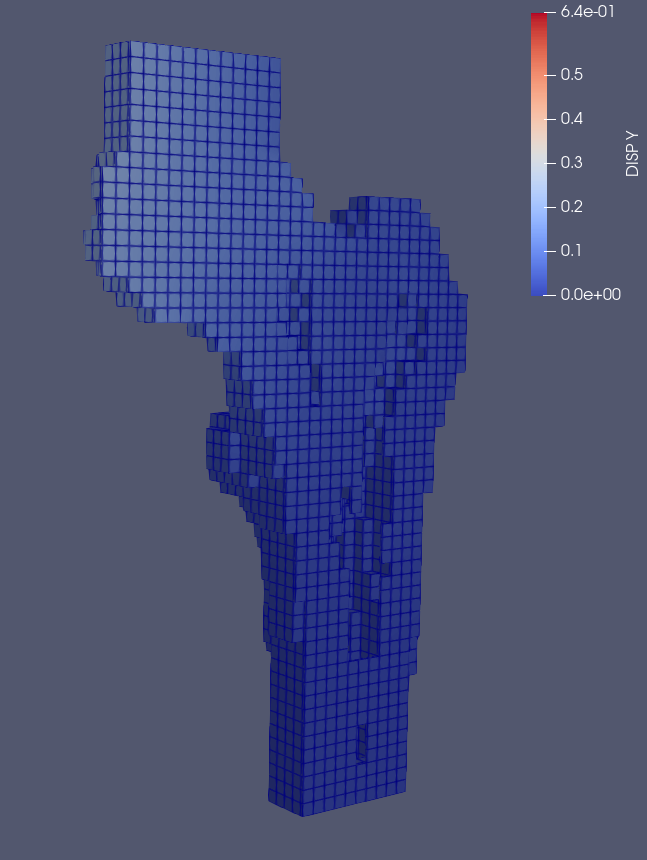
\includegraphics[width=\textwidth]{displacement-Y}
            \caption{Displacement magnitude in Y direction}
            \label{fig:displacement-Y}
        \end{minipage}
        \hfill
        \begin{minipage}[b]{0.3\textwidth}
            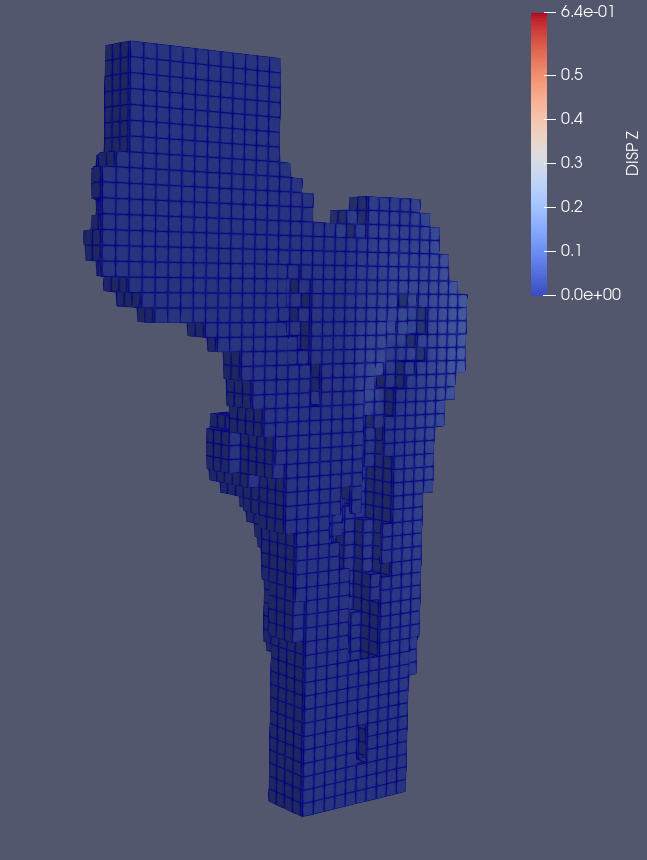
\includegraphics[width=\textwidth]{displacement-Z}
            \caption{Displacement magnitude in Z direction}
            \label{fig:displacement-Z}
        \end{minipage}
    \end{figure}

    \begin{figure}[htbp]
        \centering
        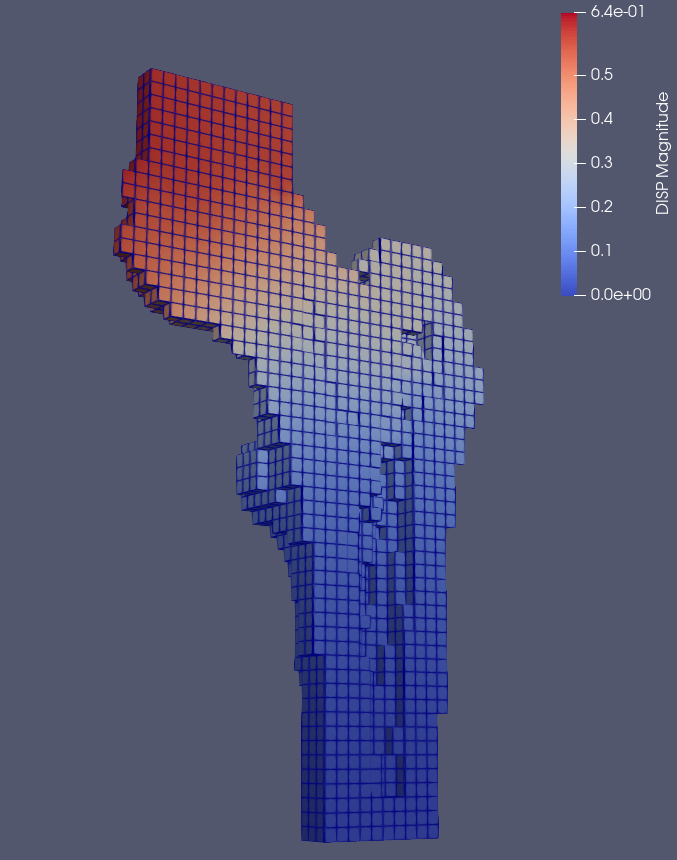
\includegraphics[width=0.5\textwidth]{displacement}
        \caption{Overall displacement magnitude}
        \label{fig:displacement}
    \end{figure}

    \vspace{10pt}
    Figure~\ref{fig:stress} depicts the von Mises stress distribution inside the bone.
    The cutting was done in such a way, to show the regions inside the bone, which are subject to the highest stress.

    \begin{figure}[htbp]
        \centering
        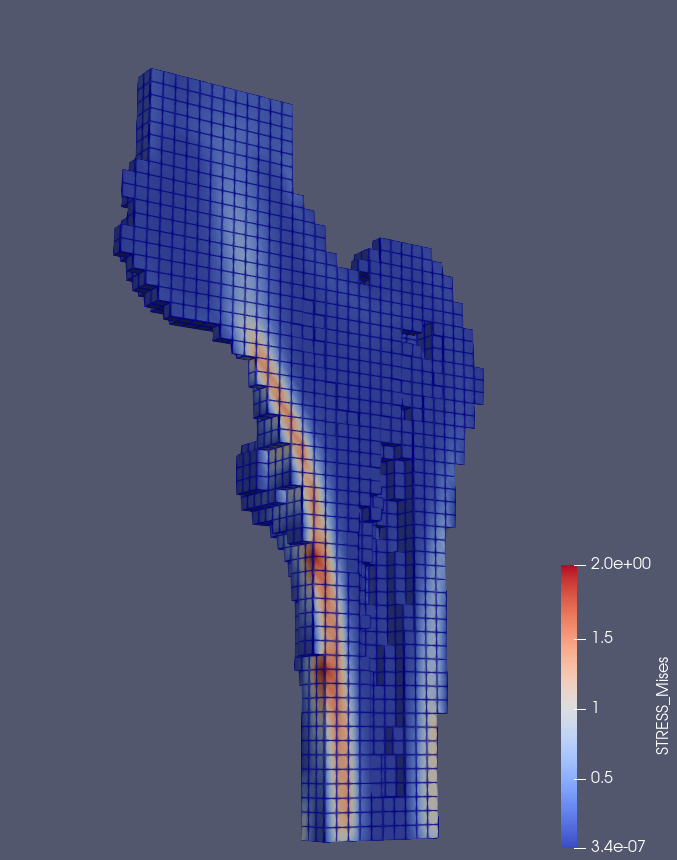
\includegraphics[width=0.5\textwidth]{stress_mises}
        \caption{von Mises stress distribution inside the bone}
        \label{fig:stress}
    \end{figure}

    \vspace{10pt}
    Table~\ref{tab:calculated_parameters} shows the calculated Spring Stiffness as well as the Average Displacement in X and Y direction at the top boundary (femoral head).
    They were calculated from the generated \texttt{model.dat} file using \texttt{Excel} to find the result of the following equations:
    \begin{equation}
        k = \frac{\sum f_z}{u_z}
    \end{equation}

    \begin{equation}
        \overline{u_x} = \frac{\sum u_x}{N_{\text{Voxel}}}
    \end{equation}

    \begin{equation}
        \overline{u_y} = \frac{\sum u_y}{N_{\text{Voxel}}}
    \end{equation}

    \begin{table}[h]
        \centering
        \begin{tabular}{|c|c|c|}
            \hline
            Parameter              & Value   & Units \\
            \hline
            Spring Stiffness       & 311.44  & N/mm  \\
            Average Displacement X & 0.47367 & mm    \\
            Average Displacement Y & 0.12804 & mm    \\
            \hline
        \end{tabular}
        \caption{Calculated parameters of the femur.}
        \label{tab:calculated_parameters}
    \end{table}


    \section{Discussion}\label{sec:discussion}
    The goal of the study was to develop a finite element model of the proximal femur to analyze the stress distribution under stance loading conditions and to evaluate the spring stiffness and displacement of the femoral head.

    \subsection{Displacement Field}\label{subsec:displacement-field}
    Looking first at the Displacement field shown in Figure~\ref{fig:displacement-X}-\ref{fig:displacement-Z}, it's clear that the majority of the displacement occurs in the positive X-direction.
    This does make intuitive sense, since the degrees of freedom are limited in the Z-direction due to the lower boundary condition and the load is applied off-axis.
    Figure~\ref{fig:displacement} shows a gradation of displacement magnitude, which seems to increase towards the femoral head.
    This pattern generally matches expectations, as the femoral head is the point of application for the displacement.
    Since the loading condition is meant to simulate a stance phase, the displacement field appears to be consistent with expected physiological behavior.

    \subsection{von Mises Stress Distribution}\label{subsec:von-mises-stress-distribution}
    The von Mises stress distribution shown in Figure~\ref{fig:stress} indicates that the highest stresses are located around the edges of the shaft as well as in the femoral neck and the intertrochanteric region, which is plausible given these areas are where the highest bending moments occur.
    The maximum stress is around $2 MPa$ which is well below the maximal stress a human femur can sustain \cite{dall2013nonlinear}, which suggests, that the absolute values of stress are plausible.

    \subsection{Spring Stiffness}\label{subsec:spring-stiffness}
    Based on Table~\ref{tab:calculated_parameters}, the spring stiffness of the proximal femur is $311.44\. N/mm$.
    Compared to literature which suggests a spring stiffness of $6.28\pm1.94\.kN/mm$, this result appears to be rather low~\cite{dall2013nonlinear}.
    There are however many factors which can influence this calculated spring stiffness.
    A few of those are:
    \begin{enumerate}
        \item Differences in the material properties, such as the Young's modulus

        \item Differences in the way the boundary conditions are applied.
        For instance, if the supports allow for more movement than would occur physiologically.

        \item If the geometry of the femur is not accurately captured, particularly the cortical and trabecular bone regions, which might happen due to the heavily decreased resolution of the model.

        \item Differences in the applied load.
        From~\cite{dall2013nonlinear} it can be seen, that the load is applied at an angle, which was not done in this analysis.
    \end{enumerate}

    \section{Conclusion}\label{sec:conclusion}
    The finite element analysis provided insights into femur biomechanics, with stress distribution aligning with physiological expectations.
    However, the calculated spring stiffness was notably lower than standard references, suggesting the need for model refinement and validation.
    This analysis illustrates the utility of computational modeling in understanding bone mechanics.

    \newpage

    \section{References}\label{sec:references}
    \begingroup
    \renewcommand{\section}[2]{}
    \bibliography{refs}
    \bibliographystyle{plain}
    \endgroup

\end{document}
